\documentclass[11pt]{article}
%\setlength {\textwidth}{180mm} 
%\setlength {\textheight}{260mm}
%\topmargin=-35.00mm
%\oddsidemargin=-10.00mm
%\pagestyle{empty}



\usepackage[toc,page]{appendix}
\usepackage{amsmath, amssymb}
\usepackage{bm}% bold math
\usepackage{cancel, caption}
\usepackage{dcolumn}% Align table columns on decimal point
\usepackage{epsfig, epsf}
\usepackage{graphicx,fancyhdr,natbib,subfigure}
\usepackage{lscape, longtable}
\usepackage{hyperref,ifthen}
\usepackage{verbatim}
\usepackage{color}
\usepackage[usenames,dvipsnames]{xcolor}
\usepackage{listings}
%% http://en.wikibooks.org/wiki/LaTeX/Colors



%%%%%%%%%%%%%%%%%%%%%%%%%%%%%%%%%%%%%%%%%%%
%       define Journal abbreviations      %
%%%%%%%%%%%%%%%%%%%%%%%%%%%%%%%%%%%%%%%%%%%
\def\nat{Nat} \def\apjl{ApJ~Lett.} \def\apj{ApJ}
\def\apjs{ApJS} \def\aj{AJ} \def\mnras{MNRAS}
\def\prd{Phys.~Rev.~D} \def\prl{Phys.~Rev.~Lett.}
\def\plb{Phys.~Lett.~B} \def\jhep{JHEP} \def\nar{NewAR}
\def\npbps{NUC.~Phys.~B~Proc.~Suppl.} \def\prep{Phys.~Rep.}
\def\pasp{PASP} \def\aap{Astron.~\&~Astrophys.} \def\araa{ARA\&A}
\def\jcap{\ref@jnl{J. Cosmology Astropart. Phys.}}%
\def\physrep{Phys.~Rep.}

\newcommand{\preep}[1]{{\tt #1} }

%%%%%%%%%%%%%%%%%%%%%%%%%%%%%%%%%%%%%%%%%%%%%%%%%%%%%
%              define symbols                       %
%%%%%%%%%%%%%%%%%%%%%%%%%%%%%%%%%%%%%%%%%%%%%%%%%%%%%
\def \Mpc {~{\rm Mpc} }
\def \Om {\Omega_0}
\def \Omb {\Omega_{\rm b}}
\def \Omcdm {\Omega_{\rm CDM}}
\def \Omlam {\Omega_{\Lambda}}
\def \Omm {\Omega_{\rm m}}
\def \ho {H_0}
\def \qo {q_0}
\def \lo {\lambda_0}
\def \kms {{\rm ~km~s}^{-1}}
\def \kmsmpc {{\rm ~km~s}^{-1}~{\rm Mpc}^{-1}}
\def \hmpc{~\;h^{-1}~{\rm Mpc}} 
\def \hkpc{\;h^{-1}{\rm kpc}} 
\def \hmpcb{h^{-1}{\rm Mpc}}
\def \dif {{\rm d}}
\def \mlim {m_{\rm l}}
\def \bj {b_{\rm J}}
\def \mb {M_{\rm b_{\rm J}}}
\def \mg {M_{\rm g}}
\def \qso {_{\rm QSO}}
\def \lrg {_{\rm LRG}}
\def \gal {_{\rm gal}}
\def \xibar {\bar{\xi}}
\def \xis{\xi(s)}
\def \xisp{\xi(\sigma, \pi)}
\def \Xisig{\Xi(\sigma)}
\def \xir{\xi(r)}
\def \max {_{\rm max}}
\def \gsim { \lower .75ex \hbox{$\sim$} \llap{\raise .27ex \hbox{$>$}} }
\def \lsim { \lower .75ex \hbox{$\sim$} \llap{\raise .27ex \hbox{$<$}} }
\def \deg {^{\circ}}
%\def \sqdeg {\rm deg^{-2}}
\def \deltac {\delta_{\rm c}}
\def \mmin {M_{\rm min}}
\def \mbh  {M_{\rm BH}}
\def \mdh  {M_{\rm DH}}
\def \msun {M_{\odot}}
\def \z {_{\rm z}}
\def \edd {_{\rm Edd}}
\def \lin {_{\rm lin}}
\def \nonlin {_{\rm non-lin}}
\def \wrms {\langle w_{\rm z}^2\rangle^{1/2}}
\def \dc {\delta_{\rm c}}
\def \wp {w_{p}(\sigma)}
\def \PwrSp {\mathcal{P}(k)}
\def \DelSq {$\Delta^{2}(k)$}
\def \WMAP {{\it WMAP \,}}
\def \cobe {{\it COBE }}
\def \COBE {{\it COBE \;}}
\def \HST  {{\it HST \,\,}}
\def \Spitzer  {{\it Spitzer \,}}
\def \ATLAS {VST-AA$\Omega$ {\it ATLAS} }
\def \BEST   {{\tt best} }
\def \TARGET {{\tt target} }
\def \TQSO   {{\tt TARGET\_QSO}}
\def \HIZ    {{\tt TARGET\_HIZ}}
\def \FIRST  {{\tt TARGET\_FIRST}}
\def \zc {z_{\rm c}}
\def \zcz {z_{\rm c,0}}

\newcommand{\ltsim}{\raisebox{-0.6ex}{$\,\stackrel
        {\raisebox{-.2ex}{$\textstyle <$}}{\sim}\,$}}
\newcommand{\gtsim}{\raisebox{-0.6ex}{$\,\stackrel
        {\raisebox{-.2ex}{$\textstyle >$}}{\sim}\,$}}
\newcommand{\simlt}{\raisebox{-0.6ex}{$\,\stackrel
        {\raisebox{-.2ex}{$\textstyle <$}}{\sim}\,$}}
\newcommand{\simgt}{\raisebox{-0.6ex}{$\,\stackrel
        {\raisebox{-.2ex}{$\textstyle >$}}{\sim}\,$}}

\newcommand{\Msun}{M_\odot}
\newcommand{\Lsun}{L_\odot}
\newcommand{\lsun}{L_\odot}
\newcommand{\Mdot}{\dot M}

\newcommand{\sqdeg}{deg$^{-2}$}
\newcommand{\lya}{Ly$\alpha$\ }
%\newcommand{\lya}{Ly\,$\alpha$\ }
\newcommand{\lyaf}{Ly\,$\alpha$\ forest}
%\newcommand{\eg}{e.g.~}
%\newcommand{\etal}{et~al.~}
\newcommand{\lyb}{Ly$\beta$\ }
\newcommand{\cii}{C\,{\sc ii}\ }
\newcommand{\ciii}{C\,{\sc iii}]\ }
\newcommand{\civ}{C\,{\sc iv}\ }
\newcommand{\SiIV}{Si\,{\sc iv}\ }
\newcommand{\mgii}{Mg\,{\sc ii}\ }
\newcommand{\feii}{Fe\,{\sc ii}\ }
\newcommand{\feiii}{Fe\,{\sc iii}\ }
\newcommand{\caii}{Ca\,{\sc ii}\ }
\newcommand{\halpha}{H\,$\alpha$\ }
\newcommand{\hbeta}{H\,$\beta$\ }
\newcommand{\hgamma}{H\,$\gamma$\ }
\newcommand{\hdelta}{H\,$\delta$\ }
\newcommand{\oi}{[O\,{\sc i}]\ }
\newcommand{\oii}{[O\,{\sc ii}]\ }
\newcommand{\oiii}{[O\,{\sc iii}]\ }
\newcommand{\heii}{[He\,{\sc ii}]\ }
\newcommand{\nv}{N\,{\sc v}\ }
\newcommand{\nev}{Ne\,{\sc v}\ }
\newcommand{\neiii}{[Ne\,{\sc iii}]\ }
\newcommand{\aliii}{Al\,{\sc iii}\ }
\newcommand{\siiii}{Si\,{\sc iii}]\ }


%%%%%%%%%%%%%%%%%%%%%%%%%%%%%%%%%%%%%%%%%%%%%%%%%%%%%
%              define Listings                       %
%%%%%%%%%%%%%%%%%%%%%%%%%%%%%%%%%%%%%%%%%%%%%%%%%%%%%
\definecolor{dkgreen}{rgb}{0,0.6,0}
\definecolor{gray}{rgb}{0.5,0.5,0.5}
\definecolor{mauve}{rgb}{0.58,0,0.82}

\lstset{frame=tb,
  language=Python,
  aboveskip=3mm,
  belowskip=3mm,
  showstringspaces=false,
  columns=flexible,
  basicstyle={\small\ttfamily},
  numbers=none,
  numberstyle=\tiny\color{gray},
  keywordstyle=\color{blue},
  commentstyle=\color{dkgreen},
  stringstyle=\color{mauve},
  breaklines=true,
  breakatwhitespace=true,
  tabsize=3
}

\begin{document}

\title{Introduction to Data Science in Python}
\author{Nicholas P. Ross}
\date{\today}
\maketitle


\begin{abstract}
Here are my (NPR's) notes on the ``Introduction to Data Science in Python''
Coursera course from the University of Michigan that I'm taking in
November 2016.  The URL for that course is\\
\href{https://www.coursera.org/learn/python-data-analysis/home/welcome}{{\tt
https://www.coursera.org/learn/python-data-analysis/home/welcome}}.
The URL for these notes is:\\
\href{https://github.com/d80b2t/Research_Notes/tree/master/Python}{\tt
https://github.com/d80b2t/Research\_Notes/tree/master/Python}
\end{abstract}


\tableofcontents


\newpage
\section{Week 1: Python Fudamentals}

\subsection{Introduction to Specialization}
Kinda a preamble!\\
General Course Outline (4 modules) \\
1. General Python Basics \\
2. The {\it pandas} Toolkit \\
3. Advanced Querying and Manipulation in {\it pandas}\\
4. Basic Statistical Analysis with {\it numpy} and {\it scipy}, and project.\\

\subsection{Syllabus}
\href{https://www.coursera.org/learn/python-data-analysis/supplement/68grE/syllabus}{\tt https://www.coursera.org/learn/python-data-analysis/supplement/68grE/syllabus}. 

If you're having problems, here are a couple of great places to go for help:
\begin{itemize}
\item{1. If the problem is with the Coursera platform such as
verification on assignments, in video quiz problems, or the Jupyter
Notebooks, please check out the Coursera Learner Support Forums.}
\item{2. If the problem deals with understanding the assignment or how
to use the Jupyter Notebooks, please read our Jupyter Notebook FAQ
page in the course resources.}
\item{3. If you have questions with the content of the course, or
questions about programming in python or with the toolkits described,
you can contact your peers and the course instructors in the
discussion forums, or go to Stack Overflow.}
\end{itemize}

\subsection{Data Science}
\href{http://drewconway.com/zia/2013/3/26/the-data-science-venn-diagram}{\tt http://drewconway.com/zia/2013/3/26/the-data-science-venn-diagram}

\begin{figure}[p]
    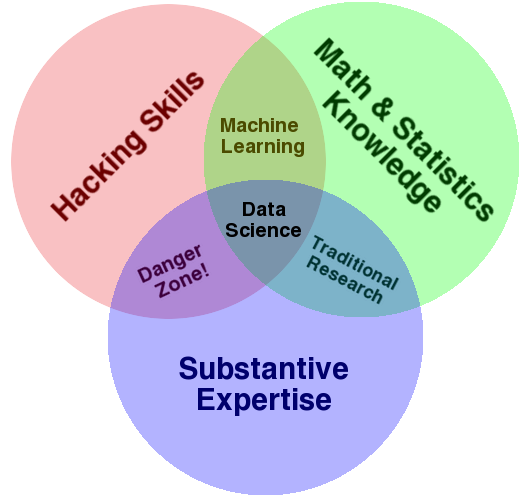
\includegraphics[width=0.8\textwidth]{Data_Science_VD.png} 
 \caption{Drew Conway's Venn Diagram.}
    \label{fig:DS_Venn}
\end{figure}

David Donoho, Professor of Statistics in Stanford., ``50 Years of Data Science''. 
1. Data Exploration and Preparation.\\
2. Data Representation and Transformation. \\
3. Computing with Data. \\
4. Data Modeling.\\
5. Data Visualization and Presentation. \\
6. Science about Data Science. \\



\subsection{The Coursera Jupyter Notebook System}
All pretty standard, straighforward. 


\subsection{Python Functions}
Of course, Python has traditional software structures like
functions. Here's an example, refactoring that previous code into a
function. You'll see the def statement indicates that we're writing a
function. Then each line that is part of the function needs to be
indented with a tab character or a couple of spaces.

\begin{lstlisting}
def add_numbers(x, y):
    return x + y

add_numbers(1, 2)
\end{lstlisting}

Okay, functions are great but they're a bit different than you might
find in other languages and here are some of subtleties
involved. First, since there's no typing, you don't have to set your
return type. Second, you don't have to use a return statement at all
actually. There's a special value called None that's returned. None is
similar to null in Java and represents the absence of value.  Third,
in Python, you can have default values for parameters.
Here's an example.
\begin{lstlisting}
def add_numbers(x,y,z=None):
    if (z==None):
        return x+y
    else:
        return x+y+z

print(add_numbers(1, 2))
print(add_numbers(1, 2, 3))
\end{lstlisting}
 In this example, we can rewrite the add numbers function to take
three parameters, but we could set the last parameter to be None by
default. This means that you can call add numbers with just two values
or with three, and you don't have to rewrite the function signature to
overload it.

\begin{lstlisting}
def do_math(a, b, kind='add'):
  if (kind=='add'):
    return a+b
  else:
    return a-b

do_math(1, 2)
\end{lstlisting}


    \subsection{Python Types and Sequences}
    The absence of static typing in Python doesn't mean that there
    aren't types. The Python language has a built in function called type
    which will show you what type of given reference is. Some of the
    common types includes strings, the type is discussed. Integers and
    floating point variables. As we've seen you can have reference as to
    function as well as a function type also exist.
    
    Typed objects have properties associated with them, and these
    properties can be data or functions. A lot of Python's built around
    different kinds of sequences or collection types. And there's three
    native kinds of collections that we're going to talk about, {\it
      tuples}, {\it lists}, and {\it dictionaries}.
    
        \subsubsection{Tuples}
        {\it A tuple is a sequence of variables which itself is immutable.}
        That means that a tuple has items in an ordering, but that it cannot
        be changed once created. We write tuples using parentheses, and we can
        mix types for the contents for the tuples. Here's a tuple which has
        four items. Two are numbers, and two are strings.
        \begin{lstlisting}
          x = (1, 'a', 2, 'b')
          type(x)
        \end{lstlisting}
        
        \subsubsection{Lists}
        Lists are very similar, but they can be mutable, so you can
        change their length, number of elements, and the element values. A
        list is declared using the square brackets.
        \begin{lstlisting}
          x = [1, 'a', 2, 'b']
          type(x)
        \end{lstlisting}
        There are a couple of different ways to change the contents of a
        list. One is through the append function which allows you to append
        new items to the end of the list.  
        \begin{lstlisting}
          x.append(3.3)
          print(x)
          \end{lstlisting}
          
        Both lists in tuple are iterable
        types, so you can write loops to go through every value they hold. The
        norm, if you want to look each item in the list is to use a {\tt for} 
        statement. This is similar to the for each loop in languages like Java
        and C\# but note that there's no typing required.
        \begin{lstlisting}
          for item in x:
          print(item)
        \end{lstlisting}

        List and tuples can also be accessed as arrays might in other
        languages, by using the square brackets operator, which is called the
        indexing operator. The first item of the list starts at position zero
        and to get the length of the list, we use the built in lan
        function. There are some other common functions that you might expect
        like min and max which will find the minimum or maximum values in a
        given list or tuple.
        \begin{lstlisting}
          i=0
          while( i != len(x) ):
              print(x[i])
              i = i + 1
          \end{lstlisting}

        \subsubsection{Other, really useful, {\tt string} stuff}
        \begin{lstlisting}
           firstname = 'Christopher'
           lastname = 'Brooks'
           print(firstname + ' ' + lastname)
           print(firstname*3)
           print('Chris' in firstname)
        \end{lstlisting}
        {\tt split} returns a list of all the words in a string, or a list split on a specific character.
        \begin{lstlisting}
          firstname = 'Christopher Arthur Hansen Brooks'.split(' ')[0] # [0] selects the first element of the list
          lastname = 'Christopher Arthur Hansen Brooks'.split(' ')[-1] # [-1] selects the last element of the list
          print(firstname)
          print(lastname)
          \end{lstlisting}


        \subsubsection{Dictionaries}
        Dictionaries are similar to lists and tuples in that they hold
        a collection of items, but they're labeled collections which do not
        have an ordering. This means that for each value you insert into the
        dictionary, you must also give a key to get that value out. In other
        languages the structure is often called a map. And in Python we use
        curly braces to denote a dictionary. Here is an example where we might
        link names to email addresses. You can see that we indicate each item
        of the dictionary when creating it using a pair of values separated by
        colons. That you can retrieve a value for a given label using the
        indexing operator.
        \begin{lstlisting}
          x = {'Christopher Brooks': 'brooksch@umich.edu', 'Bill Gates': 'billg@microsoft.com'}
          x['Christopher Brooks'] # Retrieve a value by using the indexing operator

          x['Kevyn Collins-Thompson'] = None
          x['Kevyn Collins-Thompson']

          ## Iterate over all of the keys:
          for name in x:
               print(x[name])

          brooksch@umich.edu
          None
          billg@microsoft.com

          ## Iterate over all of the values:
          for email in x.values():
              print(email)
          
         ## Iterate over all of the items in the list:

         ## You can unpack a sequence into different variables:
         x = ('Christopher', 'Brooks', 'brooksch@umich.edu')
         fname, lname, email = x
        \end{lstlisting}
        This last example is a little bit different, and it's an
        example of something called unpacking. In Python you can have
        sequence, that's a list or a tuple of values, and you can unpack those
        items into different variables through assignment in one statement.

    \subsection{Python More on Strings}
    In Python 3 strings are Unicode based, which led to the 256
    characters in ASCII.  But the world doesn't just run on Latin
    characters and there's a need to support non-English languages as well
    as characters which are not commonly used in words, but are commonly
    used elsewhere like mathematical operators. The Unicode Transformation
    Format, or UTF, is an attempt to solve this. It can be used to
    represent over a million different characters. This includes not only
    human languages like you might expect, but symbols like emojis
    too. Python 3 uses Unicode by default so there is no problem in
    dealing with international character sets.
    \begin{lstlisting}
      sales_record = {
        'price': 3.24,
        'num_items': 4,
        'person': 'Chris'}
      
      sales_statement = '{} bought {} item(s) at a price of {} each for a total of {}'
      
      print(sales_statement.format(sales_record['person'],
                                    sales_record['num_items'],
                                    sales_record['price'],
                                    sales_record['num_items']*sales_record['price']))
    \end{lstlisting}

      
\newpage
    \subsection{Python Demonstration: Reading and Writing CSV files}
    \begin{lstlisting}
      import csv
      % precision 2
      with open('mpg.csv') as csvfile:
          mpg = list(csv.DictReader(csvfile))
          
       mpg[:3] # The first three dictionaries in our list.
    \end{lstlisting}
    {\tt csv.Dictreader} has read in each row of our csv file as a
    dictionary. {\tt len} shows that our list is comprised of 234
    dictionaries.
    {\tt keys} gives us the column names of our csv:
    \begin{lstlisting}
      mpg[0].keys()
    \end{lstlisting}
    This is how to find the average cty fuel economy across all cars. All values in the dictionaries are strings, so we need to convert to float.
    \begin{lstlisting}
      sum(float(d['cty']) for d in mpg) / len(mpg)
      ## Wondering if `d' here is some universal shorthand for the dict...??
    \end{lstlisting}

    \noindent
    Here's a more complex example where we are grouping the cars by
    number of cylinder, and finding the average cty mpg for each group.
    \begin{lstlisting}
      cylinders = set(d['cyl'] for d in mpg)
      cylinders
      
      CtyMpgByCyl = []
      
      for c in cylinders: # iterate over all the cylinder levels
          summpg = 0
          cyltypecount = 0
          for d in mpg: # iterate over all dictionaries
              if d['cyl'] == c: # if the cylinder level type matches,
                  summpg += float(d['cty']) # add the cty mpg
                  cyltypecount += 1 # increment the count

          CtyMpgByCyl.append((c, summpg / cyltypecount)) # append the tuple ('cylinder', 'avg mpg')

      CtyMpgByCyl.sort(key=lambda x: x[0])
      CtyMpgByCyl
     \end{lstlisting}

    \subsection{Python Dates and Times}
     \begin{lstlisting}
       import datetime as dt
       import time as tm

       # time returns the current time in seconds since the Epoch. (January 1st, 1970)
       tm.time()
       
       # Convert the timestamp to datetime.
       dtnow = dt.datetime.fromtimestamp(tm.time())
       dtnow

       # get year, month, day, etc.from a datetime
       dtnow.year, dtnow.month, dtnow.day, dtnow.hour, dtnow.minute, dtnow.second 

       # create a timedelta of 100 days
       delta = dt.timedelta(days = 100)  
       delta

       today = dt.date.today()
       
       today - delta # the date 100 days ago

       datetime.date(2016, 8, 7)

       today > today-delta # compare dates
     \end{lstlisting}


    \newpage
    \subsection{Advanced Python Objects, map()}
    Tiny, wee intro to OOP. 

    \noindent
    You can define a class using a class keyword, and ending with a
    colon.  Anything indented below this, is within the scope of the
    class. An example of a class in python:
    \begin{lstlisting}
      class Person:
          department = 'School of Information'   # a class variable
      
          def set_name(self, new_name):             # a method
              self.name = new_name
          def set_location(self, new_location):
              self.location = new_location
    \end{lstlisting}
    Classes in Python are generally named using camel case, which
    means the first character of each word is capitalized.

    \smallskip\smallskip\noindent
    You don't declare variables within the object, you just start
    using them. Class variables can also be declared. These are just
    variables which are shared across all instances. So in this example,
    we're saying that the default for all people is at the school of
    information.
    
    \smallskip\smallskip\noindent
    To define a {\it method}, you just write it as you would have a
    function. The one change, is that to have access to the instance which
    a method is being invoked upon, you must include {\tt self}, in the
    method signature. Similarly, if you want to refer to instance
    variables set on the object, you pre-pen them with the word {\tt
      self}, with a full stop. In this definition of a person, for instance,
    we have written two methods, {\tt set\_name} and {\tt
      set\_location}. And both change instance bound variables, called name
    and location respectively.
    
    \smallskip\smallskip\noindent
    Couple of key points on Python objects. First, objects in Python
    do not have private or protected member. If you instantiate an object,
    you have full access to any of the methods or attributes of that
    object. Second, there's no need for an explicit constructor when
    creating objects in Python. You can add a constructor if you want to
    by declaring the double underscore init double underscore method.

    \smallskip\smallskip\noindent
    {\tt map()}.\\
    So, Functional programming is a programming paradigm in which you
    explicitly declare all parameters which could change through execution
    of a given function. Thus functional programming is referred to as
    being ``side-effect free'', because there is a software contract that
    describes what can actually change by calling a function. Now, Python
    isn't a functional programming language in the pure sense. Since you
    can have many side effects of functions, and certainly you don't have
    to pass in the parameters of everything that you're interested in
    changing.
    
    But functional programming causes one to think more heavily while
    chaining operations together. And this really is a sort of underlying
    theme in much of data science and date cleaning in particular. So,
    functional programming methods are often used in Python, and it's not
    uncommon to see a parameter for a function, be a function itself. The
    map built-in function is one example of a functional programming
    feature of Python, that I think ties together a number of aspects of
    the language. The map function signature looks like this. The first
    parameters of function that you want executed, and the second
    parameter, and every following parameter, is something which can be
    iterated upon.

    \begin{lstlisting}
      store1 = [10.00, 11.00, 12.34, 2.34]
      store2 = [9.00, 11.10, 12.34, 2.01]
      cheapest = map(min, store1, store2)
      cheapest

      <map at 0x7fd424086eb8>
    \end{lstlisting}
    But when we go to print out the map, we see that we get an odd
    reference value instead of a list of items that we're expecting. This
    is called lazy evaluation. In Python, the map function returns to you
    a mapped object. Maps are iterable, just like lists and tuples, so we
    can use a for loop to look at all of the values in the map.

    \begin{lstlisting}
      for item in cheapest:
          print(item)
    \end{lstlisting}
    then gives you understandable O/P. 

    \newpage
    \medskip\medskip
    \noindent
    Here is a list of faculty teaching this MOOC. Can you write a
    function and apply it using map() to get a list of all faculty titles
    and last names (e.g. ['Dr. Brooks', 'Dr. Collins-Thompson', ....])??
    \begin{lstlisting}
      people = ['Dr. Christopher Brooks', 'Dr. Kevyn Collins-Thompson', 'Dr. VG Vinod Vydiswaran', 'Dr. Daniel Romero']
      
      def split_title_and_name(person):
          return #Your answer here

      list(map(#Your answer here))
    \end{lstlisting}

    \noindent 
    with an answer looking something like:
    \begin{lstlisting}
     people = ['Dr. Christopher Brooks', 'Dr. Kevyn Collins-Thompson', 'Dr. VG Vinod Vydiswaran', 'Dr. Daniel Romero']
      
     def split_title_and_name(person):
         title = person.split()[0]
         lastname = person.split()[-1]
         return '{} {}'.format(title, lastname)

     list(map(split_title_and_name, people))
    \end{lstlisting}
    giving:
    \begin{lstlisting}
    ['Dr. Brooks', 'Dr. Collins-Thompson', 'Dr. Vydiswaran', 'Dr. Romero']
    \end{lstlisting}


    \newpage
    \subsection{Advanced Python Lambda and List Comprehensions}
    Lambda's are Python's way of creating anonymous functions. These are the same as other functions, but they have no name. The intent is that they're simple or short lived and it's easier just to write out the function in one line instead of going to the trouble of creating a named function.
    
    \smallskip \smallskip \noindent
    Convert this function in a lambda:
    \begin{lstlisting}
      people = ['Dr. Christopher Brooks', 'Dr. Kevyn Collins-Thompson', 'Dr. VG Vinod Vydiswaran', 'Dr. Daniel Romero']

      def split_title_and_name(person):
          return person.split()[0] + ' ' + person.split()[-1]
      
          #option 1
          for person in people:
              print(split_title_and_name(person) == (lambda person:???))

              #option 2
              #list(map(split_title_and_name, people)) == list(map(???))
    \end{lstlisting}

    Something like this works well...
    \begin{lstlisting}
      people = ['Dr. Christopher Brooks', 'Dr. Kevyn Collins-Thompson', 'Dr. VG Vinod Vydiswaran', 'Dr. Daniel Romero']
      
      def split_title_and_name(person):
          return person.split()[0] + ' ' + person.split()[-1]
      
          #option 1
          for person in people:
              print(split_title_and_name(person) == (lambda x: x.split()[0] + ' ' + x.split()[-1])(person))

          #option 2
          list(map(split_title_and_name, people)) == list(map(lambda person: person.split()[0] + ' ' + person.split()[-1], people))
    \end{lstlisting}
    Noting the double ``=='' signs just to check the logic (vs. actually printing something out). 


    \smallskip     \smallskip \noindent
    {\bf List Comprehensions.}\\
    \begin{lstlisting}
      my_list = []
      for number in range(0, 1000):
          if number % 2 == 0:
              my_list.append(number)
     my_list
    \end{lstlisting}
      vs. 

    \begin{lstlisting}
      my_list = [number for number in range(0,1000) if number % 2 == 0]
      my_list
    \end{lstlisting}

    Exercise: Convert function into a lise comprehension:
    \begin{lstlisting}
      def times_tables():
          lst = []
          for i in range(10):
              for j in range (10):
                  lst.append(i*j)
          return lst
      
      times_tables() == [???]
    \end{lstlisting}

    \begin{lstlisting}
      def times_tables():
          lst = []
          for i in range(10):
              for j in range (10):
                  lst.append(i*j)
          return lst

      times_tables() == [j*i for i in range(10) for j in range(10)]
    \end{lstlisting}
    Noting the double ``=='' signs just to check the logic (vs. actually printing something out). 


    \newpage    
    \subsection{Advanced Python Demonstration: The Numerical Python Library (Numpy)}
    \begin{lstlisting}
      ## Difference between 
      np.array([1, 2, 3] * 3) 
      np.repeat([1, 2, 3], 3)
    \end{lstlisting}

    \begin{lstlisting}
      a = np.array([-4, -2, 1, 3, 5])
      a.sum()
      a.max()
      a.min()
      a.mean()
      a.std
      ## argmax and argmin return the index of the maximum and minimum values in the array
      a.argmax()
      a.argmin()
    \end{lstlisting}


    \begin{lstlisting}
      test = np.random.randint(0, 10, (4,3))
      test
      array(
      [[8, 5, 3],
       [6, 0, 8],
       [3, 0, 0],
       [1, 8, 0]])

       test[0]
       array([8, 5, 3])

       test[0][0]
       8

       test[0,0]
       8

       test[1]
       array([6, 0, 8])

       test[0][1]
       5

       test[0, 1]
       5

       for i, row in enumerate(test):
           print('row', i, 'is', row)
           
       row 0 is [8 5 3]
       row 1 is [6 0 8]
       row 2 is [3 0 0]
       row 3 is [1 8 0]

       # Use `zip` to iterate over multiple iterables.

       test2 = test**2
       for i, j in zip(test, test2):
           print(i,'+',j,'=',i+j)
       
       [8 5 3] + [64 25  9] = [72 30 12]
       [6 0 8] + [36  0 64] = [42  0 72]
       [3 0 0] + [9 0 0] = [12  0  0]
       [1 8 0] + [ 1 64  0] = [ 2 72  0]
    \end{lstlisting}

Week One quiz notes:
Python is an example of an Interpreted language. \\
In Python, strings are considered INmutable.\\
When you create a lambda, what type is returned? A function.\\







%%%%%%%%%%%%%%%%%%%%%%%%%%%%%%%%%%%%%%%%%%%%%%%%%%%%%%%%%%%
%%%%%%%%%%%%%%%%%%%%%%%%%%%%%%%%%%%%%%%%%%%%%%%%%%%%%%%%%%%
%%
%%
%%    W E E K     T W O    
%%
%%
%%%%%%%%%%%%%%%%%%%%%%%%%%%%%%%%%%%%%%%%%%%%%%%%%%%%%%%%%%%
%%%%%%%%%%%%%%%%%%%%%%%%%%%%%%%%%%%%%%%%%%%%%%%%%%%%%%%%%%%
\newpage
\section{Week Two: Basic Data Processing with Pandas}

    \subsection{Introduction}
    GoTo:  \href{StackOverflow}{http://stackoverflow.com/}. \\
    Good RSS: \href{http://planetpython.org/}{Planet Python}. \\
    Podcast: {\href http://dataskeptic.com/}{http://dataskeptic.com/}\\


    \subsection{The Series Data Structure}
    
    \smallskip\smallskip\noindent
    {\tt pd.Series(data=None, index=None, dtype=None, name=None, copy=False, fastpath=False)}

    \smallskip\smallskip\noindent
    If we create a list of strings and we have one element, a None
    type, pandas inserts it as a None and uses the type object for the
    underlying array:
    \begin{lstlisting}
      animals = ['Tiger', 'Bear', None]
      print(type(pd.Series(animals)))
      pd.Series(animals)
      
      <class 'pandas.core.series.Series'>

      0    Tiger
      1    Bear
      2    None
      dtype: object
    \end{lstlisting}
    
    \smallskip\smallskip\noindent
    If we create a list of numbers, integers or floats, and put in the
    None type, pandas automatically converts this to a special floating
    point value designated as NAN, which stands for not a number:
    \begin{lstlisting}
      numbers = [1, 2, None]
      print(type(pd.Series(numbers)))
      pd.Series(numbers)

      <class 'pandas.core.series.Series'>

      0    1.0
      1    2.0
      2    NaN
      dtype: float64
    \end{lstlisting}
    {\it N.B the NaN; {\bf NAN is not none and when we try the equality test, it's false.}}

    \begin{lstlisting}
     import numpy as np
     np.nan == None
     False

     np.nan == np.nan
     False  # Watch Out!!!!

     np.isnan(np.nan)
     True
    \end{lstlisting}

    What happens if your list of values in the index object are not aligned with the keys in your dictionary for creating the series? Well, pandas overrides the automatic creation to favor only and all of the indices values that you provided. So it will ignore it from your dictionary, all keys, which are not in your index, and pandas will add non type or NAN values for any index value you provide, which is not in your dictionary key list. e.g.:
    \begin{lstlisting}
    sports = {'Archery': 'Bhutan',
          'Golf': 'Scotland',
          'Sumo': 'Japan',
          'Taekwondo': 'South Korea'}
        s = pd.Series(sports, index=['Golf', 'Sumo', 'Hockey'])
        s
        
        Golf      Scotland
        Sumo         Japan
        Hockey         NaN
        dtype: object
    \end{lstlisting}


    \subsection{Querying a Series}
    \smallskip \smallskip \noindent
    A panda.Series can be queried, either by the index position or the
    index label. As we saw, if you don't give an index to the series, the
    position and the label are effectively the same values. To query by
    numeric location, starting at zero, use the iloc attribute. To query
    by the index label, you can use the loc attribute.

    \smallskip \smallskip \noindent
    Keep in mind that iloc and loc are not methods, they are
    attributes. So you don't use parentheses to query them, but square
    brackets instead, which we'll call the indexing operator. Though in
    Python, this calls get and set an item methods depending on the
    context of its use.

    \begin{lstlisting}
      sports = {99: 'Bhutan',
                     100: 'Scotland',
                     101: 'Japan',
                     102: 'South Korea'}
      s = pd.Series(sports)

      s[0] 
      # Gives a KeyError!!! Use instead:
      s.iloc[0]
        
      'Bhutan'
    \end{lstlisting}
    
    Slow...
    \begin{lstlisting}
    total = 0
    for item in s:
        total+=item
        print(total)
    \end{lstlisting}

    \begin{lstlisting}
     import numpy as np
     
     total = np.sum(s)
     print(total)
    \end{lstlisting}

    \begin{lstlisting}
    #this creates a big series of random numbers
    s = pd.Series(np.random.randint(0,10000,10000))
    s.head()
    
    %%timeit -n 100
    summary = 0
    for item in s:
        summary+=item
    100 loops, best of 3: 1.7 ms per loop
       
    %%timeit -n 100
    summary = np.sum(s)    
    100 loops, best of 3: 164 µs per loop
    \end{lstlisting}

    \smallskip\smallskip\noindent
    Up until now I've shown only examples of a series where the index
    values were unique. I want to end this lecture by showing an example
    where index values are not unique, and this makes data frames
    different, conceptually, that a relational database might be. 

    Revisiting the issue of countries and their national sports, it
    turns out that many countries seem to like this game cricket. We go
    back to our original series on sports. It's possible to create a new
    series object with multiple entries for cricket, and then use append
    to bring these together. There are a couple of important
    considerations when using append. First, Pandas is going to take your
    series and try to infer the best data types to use. In this example,
    everything is a string, so there's no problems here.
    
    Second, the append method doesn't actually change the underlying
    series. It instead returns a new series which is made up of the two
    appended together. We can see this by going back and printing the
    original series of values and seeing that they haven't changed.\\
    ...\\
    ...\\
    ...\\

    \smallskip\smallskip\noindent
    In this lecture, we focused on one of the primary data types of
    the Pandas library, the series. There are many more methods associated
    with this series object that we haven't talked about. But with these
    basics down, we'll move on to talking about the Panda's
    two-dimensional data structure, the data frame. The data frame is very
    similar to the series object, but includes multiple columns of data,
    and is the structure that you'll spend the majority of your time
    working with when cleaning and aggregating data.  


    \subsection{The DataFrame Data Structure}
    \smallskip\smallskip\noindent
    {\bf N.B.} Since {\tt iloc} and {\tt loc} are used for row
    selection, the Panda's developers reserved indexing operator directly
    on the DataFrame for column selection. In a Panda's DataFrame, columns
    always have a name.

    As we saw, {\tt .loc} does row selection, and it can take two
    parameters, the row index and the list of column names. {\tt .loc} also
    supports slicing. If we wanted to select all rows, we can use a column
    to indicate a full slice from beginning to end. And then add the
    column name as the second parameter as a string. In fact, if we wanted
    to include multiply columns, we could do so in a list. And Pandas will
    bring back only the columns we have asked for. Here's an example,
    where we ask for all of the name and cost values for all stores using
    the {\tt .loc} operator. e.g.  
    \begin{lstlisting}
      df['Cost']
      
      df.loc['Store 1']['Cost']
      
      df.loc[:,['Name', 'Cost']]
    \end{lstlisting}
    Also, consider the issue of chaining carefully, and try to avoid
    it, it can cause unpredictable results. Where your intent was to
    obtain a view of the data, but instead Pandas returns to you a
    copy. In the Panda's world, friends don't let friends chain calls. So
    if you see it, point it out, and share a less ambiguous solution.

    Also, consider the issue of chaining carefully, and try to avoid
    it, it can cause unpredictable results. Where your intent was to
    obtain a view of the data, but instead Pandas returns to you a
    copy. In the Panda's world, friends don't let friends chain calls. So
    if you see it, point it out, and share a less ambiguous solution.
    \begin{lstlisting}
      df['Location'] = None
      df
      
      # Update the Cost column with a 20\% discount.
      df['Cost'] = df['Cost'] * 0.8   
      # or... 
      df['Cost'] *= 0.8
    \end{lstlisting}


    \subsection{DataFrame Indexing and Loading}
    \smallskip     \smallskip     \noindent
    Pandas has built-in support for delimited files such as CSV files
    as well as a variety of other data formats including relational
    databases Excel and HTML tables.  I've saved a CSV file called
    olympics.csv, which has data from Wikipedia that contains a summary
    list of the medal various countries have won at the Olympics.
    
    \smallskip     \smallskip     \noindent
    We can take a look at this file using the shell command cat. Which
    we can invoke directly using the exclamation point.
    \begin{lstlisting}
      !cat olympics.csv
      df = pd.read_csv('olympics.csv', index_col = 0, skiprows=1)
      df.head()
    \end{lstlisting}


    \subsection{Querying a DataFrame}
    \smallskip     \smallskip     \noindent
    {\bf This is all very close to the ol' IDL Where function...  :-) }
    
    \smallskip     \smallskip     \noindent
    One more thing to keep in mind if you're not used to Boolean or
    bit masking for data reduction. The output of two Boolean masks being
    compared with logical operators is another Boolean mask. This means
    that you can chain together a bunch of and/or statements in order to
    create more complex queries, and the result is a single Boolean mask. 

    For instance, we could create a mask for all of those countries
    who have received a gold in the summer Olympics and logically order
    that with all of those countries who have received a gold in the
    winter Olympics. If we apply this to the data frame and use the length
    function to see how many rows there are, we see that there are 101
    countries which have won a gold metal at some time.
    
    Another example for fun. Have there been any countries who have
    only won a gold in the winter Olympics and never in the summer
    Olympics? Here's one way to answer that.  Poor
    Liechtenstein. Thankfully the Olympics come every four years. I know
    who I'll be cheering for in 2020 to win their first summer gold.
    
    Extremely important, and often an issue for new users, is to remember
    that each Boolean mask needs to be encased in parenthesis because of
    the order of operations. This can cause no end of frustration if
    you're not used to it, so be careful.
    \begin{lstlisting}
      only_gold = df.where(df['Gold'] > 0)
      
      only_gold = only_gold.dropna()
      
      only_gold = df[df['Gold'] > 0]
      
      len(df[(df['Gold'] > 0) | (df['Gold.1'] > 0)])
      
      df[(df['Gold.1'] > 0) & (df['Gold'] == 0)]
    \end{lstlisting}

    Write a query to return all the names of people who bought products worth more than \$3.00.
    \begin{lstlisting}
     purchase_1 = pd.Series({'Name': 'Chris',
                                             'Item Purchased': 'Dog Food',
                                             'Cost': 22.50})
     purchase_2 = pd.Series({'Name': 'Kevyn',
                                            'Item Purchased': 'Kitty Litter',
                                            'Cost': 2.50})
     purchase_3 = pd.Series({'Name': 'Vinod',
                                            'Item Purchased': 'Bird Seed',
                                            'Cost': 5.00})

     df = pd.DataFrame([purchase_1, purchase_2, purchase_3], index=['Store 1', 'Store 1', 'Store 2'])
     
    # df['Name'[df['Cost'] >3.00]] does not work...

    df['Name'][df['Cost']>3.0]
    \end{lstlisting}

     
    \subsection{Indexing Dataframes}

    \begin{lstlisting}
      df['country'] = df.index
      ##  manually create a new column and copy into it values from the index attribute. 
      ##  (preserve the country information into a new column)

      df = df.set_index('Gold')

      df = df.reset_index()
      # We can get rid of the ``blank'' entries by calling reset_index
    \end{lstlisting}

    Pandas can do multi-level indexing. 
    \begin{lstlisting}
     df = pd.read_csv('census.csv')
     df['SUMLEV'].unique()
     df=df[df['SUMLEV'] == 50]    #Careful, this is ``destructive''....
     columns_to_keep = ['STNAME',
                                      'CTYNAME',
                                      'BIRTHS2010',
                                      'BIRTHS2011, 
                                      ....
                                      'POPESTIMATE2014',
                                      'POPESTIMATE2015']
    df = df[columns_to_keep]

    df = df.set_index(['STNAME', 'CTYNAME'])
    \end{lstlisting}
    When you use a multi-index, you must provide the arguments in
    order by the level you wish to query. Inside of the index, each column
    is called a level and the outermost column is level zero. For
    instance, if we want to see the population results from Washenaw
    county...
    \begin{lstlisting}
      df.loc['Michigan', 'Washtenaw County']
      
      df.loc[ [('Michigan', 'Washtenaw County'),
                  ('Michigan', 'Wayne County')] ]
    \end{lstlisting}
    
    Reindex the purchase records DataFrame to be indexed
    hierarchically, first by store, then by person. Name these indexes
    ``Location'' and ``Name''. Then add a new entry to it with the value
    of: 
    {\tt Name: 'Kevyn', Item Purchased: 'Kitty Food', Cost: 3.00 Location': 'Store 2'.}
    \begin{lstlisting}
      purchase_1 = pd.Series({'Name': 'Chris',
                                             'Item Purchased': 'Dog Food',
                                             'Cost': 22.50})
      purchase_2 = pd.Series({'Name': 'Kevyn',
                                             'Item Purchased': 'Kitty Litter',
                                             'Cost': 2.50})
      purchase_3 = pd.Series({'Name': 'Vinod',
                                             'Item Purchased': 'Bird Seed',
                                             'Cost': 5.00})

      df = pd.DataFrame([purchase_1, purchase_2, purchase_3], index=['Store 1', 'Store 1', 'Store 2'])

      # Your answer here
      df = df.set_index([df.index, 'Name'])
      df.index.names = ['Location', 'Name']
      df = df.append(pd.Series(data={'Cost': 3.00, 'Item Purchased': 'Kitty Food'}, name=('Store 2', 'Kevyn')))
df
    \end{lstlisting}


    \subsection{Missing Values}
    \begin{lstlisting}
      df.fillna?

      ## Promote the time stamp to an index, then sort on the index. 
      df = df.set_index('time')
      df = df.sort_index()

      ## Reset the index, using some multi-level indexing instead,
      ## promote the user name to a second level of the index
      df = df.reset_index()
      df = df.set_index(['time', 'user'])

      df = df.fillna(method='ffill')
    \end{lstlisting}

































\newpage
\section{Week Three}

    \subsection{Merging Dataframes}
    \subsection{Pandas Idioms}
    \subsection{Group by}
    \subsection{Scales}
    \subsection{Pivot Tables}
    \subsection{Date Functionality}




\newpage
\section{Week Four: Statistical Analysis in Python and Project}
    \subsection{Introduction}
    \subsection{Distributions}
    \subsection{More Distributions}
    \subsection{Hypothesis Testing in Python}

    %Discussion Prompt: The End of Theory35 min
    %Discussion Prompt: Science Isn't Broken: p-hacking activity45 min
    %Week 4 Slides


















\section{References and Bibliography}




\bibliographystyle{mn2e}
\bibliography{/cos_pc19a_npr/LaTeX/tester_mnras}

\end{document}

